%% generated by python/export_paired_panels.py
%% sweeps: 2026-10-02-paper, GNvpro top-up; commit 259ce29
%   (a) $[-1,1]$ over $[0,T]$, DCR, Hamiltonian, Adam, $T{=}10$: ratio 0.047 [0.036, 0.060], first lower on 10 of 10, seed spread 1.442
%   (b) Legendre over monomial, ELM, Hamiltonian, GNvpro, $T{=}1$: ratio 0.993 [0.984, 1.002], first lower on 8 of 10, seed spread 1.021
%   (c) Legendre over monomial, DCR, Hamiltonian, GNvpro, $T{=}1$: ratio 1.027 [0.843, 1.252], first lower on 5 of 10, seed spread 1.286
\documentclass[tikz]{standalone}
\usepackage{pgfplots}
\usepgfplotslibrary{groupplots}
\pgfplotsset{compat=1.18}
\definecolor{bandblue}{rgb}{0.10,0.32,0.72}
\begin{document}
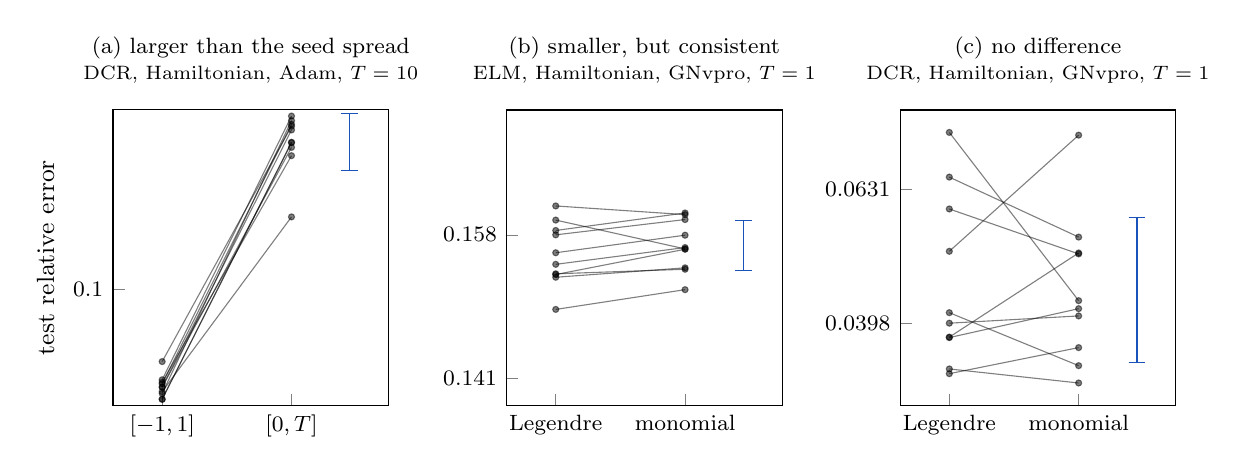
\begin{tikzpicture}
\begin{groupplot}[group style={group size=3 by 1,horizontal sep=1.5cm},
  width=2.0in,height=2.1in,ymode=log,
  log ticks with fixed point,
  xmin=0.62,xmax=2.75,xtick={1,2},
  title style={font=\footnotesize,align=center},
  tick label style={font=\footnotesize},label style={font=\small},
  ytick pos=left,xtick pos=bottom,clip=false]
\nextgroupplot[title={(a) larger than the seed spread\\{\scriptsize DCR, Hamiltonian, Adam, $T=10$}},xticklabels={{$[-1,1]$},{$[0,T]$}},ymin=0.0232303,ymax=0.943133,ylabel={test relative error}]
\addplot[color=black,opacity=0.5,line width=0.4pt,mark=*,mark size=1.1pt] coordinates {(1,0.0292412) (2,0.73398)};
\addplot[color=black,opacity=0.5,line width=0.4pt,mark=*,mark size=1.1pt] coordinates {(1,0.0320373) (2,0.873271)};
\addplot[color=black,opacity=0.5,line width=0.4pt,mark=*,mark size=1.1pt] coordinates {(1,0.0304724) (2,0.788402)};
\addplot[color=black,opacity=0.5,line width=0.4pt,mark=*,mark size=1.1pt] coordinates {(1,0.0250887) (2,0.629162)};
\addplot[color=black,opacity=0.5,line width=0.4pt,mark=*,mark size=1.1pt] coordinates {(1,0.0275882) (2,0.246763)};
\addplot[color=black,opacity=0.5,line width=0.4pt,mark=*,mark size=1.1pt] coordinates {(1,0.0269872) (2,0.825239)};
\addplot[color=black,opacity=0.5,line width=0.4pt,mark=*,mark size=1.1pt] coordinates {(1,0.029177) (2,0.589726)};
\addplot[color=black,opacity=0.5,line width=0.4pt,mark=*,mark size=1.1pt] coordinates {(1,0.0310259) (2,0.531593)};
\addplot[color=black,opacity=0.5,line width=0.4pt,mark=*,mark size=1.1pt] coordinates {(1,0.0250956) (2,0.625362)};
\addplot[color=black,opacity=0.5,line width=0.4pt,mark=*,mark size=1.1pt] coordinates {(1,0.0402525) (2,0.769239)};
\draw[bandblue,|-|,line width=0.5pt] (axis cs:2.45,0.436581) -- (axis cs:2.45,0.907528);
\nextgroupplot[title={(b) smaller, but consistent\\{\scriptsize ELM, Hamiltonian, GNvpro, $T=1$}},xticklabels={{Legendre},{monomial}},ymin=0.138225,ymax=0.175147]
\addplot[color=black,opacity=0.5,line width=0.4pt,mark=*,mark size=1.1pt] coordinates {(1,0.162173) (2,0.161063)};
\addplot[color=black,opacity=0.5,line width=0.4pt,mark=*,mark size=1.1pt] coordinates {(1,0.149283) (2,0.151666)};
\addplot[color=black,opacity=0.5,line width=0.4pt,mark=*,mark size=1.1pt] coordinates {(1,0.154771) (2,0.156865)};
\addplot[color=black,opacity=0.5,line width=0.4pt,mark=*,mark size=1.1pt] coordinates {(1,0.153598) (2,0.15416)};
\addplot[color=black,opacity=0.5,line width=0.4pt,mark=*,mark size=1.1pt] coordinates {(1,0.153181) (2,0.154331)};
\addplot[color=black,opacity=0.5,line width=0.4pt,mark=*,mark size=1.1pt] coordinates {(1,0.158477) (2,0.160418)};
\addplot[color=black,opacity=0.5,line width=0.4pt,mark=*,mark size=1.1pt] coordinates {(1,0.160361) (2,0.156692)};
\addplot[color=black,opacity=0.5,line width=0.4pt,mark=*,mark size=1.1pt] coordinates {(1,0.15351) (2,0.156648)};
\addplot[color=black,opacity=0.5,line width=0.4pt,mark=*,mark size=1.1pt] coordinates {(1,0.159026) (2,0.161279)};
\addplot[color=black,opacity=0.5,line width=0.4pt,mark=*,mark size=1.1pt] coordinates {(1,0.156213) (2,0.158431)};
\draw[bandblue,|-|,line width=0.5pt] (axis cs:2.45,0.153953) -- (axis cs:2.45,0.160365);
\nextgroupplot[title={(c) no difference\\{\scriptsize DCR, Hamiltonian, GNvpro, $T=1$}},xticklabels={{Legendre},{monomial}},ymin=0.0300636,ymax=0.0828714]
\addplot[color=black,opacity=0.5,line width=0.4pt,mark=*,mark size=1.1pt] coordinates {(1,0.0767328) (2,0.043068)};
\addplot[color=black,opacity=0.5,line width=0.4pt,mark=*,mark size=1.1pt] coordinates {(1,0.0380051) (2,0.0507334)};
\addplot[color=black,opacity=0.5,line width=0.4pt,mark=*,mark size=1.1pt] coordinates {(1,0.0589955) (2,0.0505631)};
\addplot[color=black,opacity=0.5,line width=0.4pt,mark=*,mark size=1.1pt] coordinates {(1,0.0340714) (2,0.0324687)};
\addplot[color=black,opacity=0.5,line width=0.4pt,mark=*,mark size=1.1pt] coordinates {(1,0.0335225) (2,0.0366609)};
\addplot[color=black,opacity=0.5,line width=0.4pt,mark=*,mark size=1.1pt] coordinates {(1,0.0658202) (2,0.0535661)};
\addplot[color=black,opacity=0.5,line width=0.4pt,mark=*,mark size=1.1pt] coordinates {(1,0.0413287) (2,0.0344583)};
\addplot[color=black,opacity=0.5,line width=0.4pt,mark=*,mark size=1.1pt] coordinates {(1,0.0379483) (2,0.0419013)};
\addplot[color=black,opacity=0.5,line width=0.4pt,mark=*,mark size=1.1pt] coordinates {(1,0.0398722) (2,0.0408682)};
\addplot[color=black,opacity=0.5,line width=0.4pt,mark=*,mark size=1.1pt] coordinates {(1,0.0510177) (2,0.0760149)};
\draw[bandblue,|-|,line width=0.5pt] (axis cs:2.45,0.0347372) -- (axis cs:2.45,0.0574294);
\end{groupplot}
\end{tikzpicture}
\end{document}
